%!TEX root=dslrob.tex

\section{Implementing a robotics application}
\label{sec:implementing}

The \diaspec{} compiler generates a programming framework with respect
to a set of declarations for entity classes, context operators and
control operators (Figure~\ref{fig:diaspec-process}). For each
component description (entity or operator) the compiler generates an
abstract class. The abstract methods in this class represent code to
be provided by the developer (\emph{hole} in
Figure~\ref{fig:diaspec-process}), to allow him to program the
application logic (\eg{} to trigger an entity action) (\textit{bump}
in Figure~\ref{fig:diaspec-process}).

\begin{figure}
  \centering
  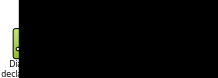
\includegraphics[width=.8\linewidth]{diaspec-process}
  \caption{Overview of the \diaspec{} development process}
  \label{fig:diaspec-process}
\end{figure}

Implementing a \diaspec{} component is done by \textit{sub-classing}
the corresponding generated abstract class. In doing so, the developer
is required to implement each abstract method. The developer writes
the application code in subclasses, not in the generated abstract
classes. This strategy contrasts with generating incomplete source
code, to be filled by the developer. As a result, in our approach, one
can change the \diaspec{} description and generate a new programming
framework without overriding the developer's code. The mismatches
between the existing code and the new programming framework are
revealed by the Java compiler. To facilitate the implementation
process, most Java IDEs are capable of generating class templates
based on super abstract classes.

In this section, we give an overview of how to implement some parts of
the case study. For a more detailed description, we refer to our
previous works~\cite{Cass09b,Cass11a,Cass11b}.

\subsection{Implementing an operator}

For each context or control operator, a dedicated abstract class is
generated in the programming framework. For each input source of this
operator, the generated abstract class contains an \emph{abstract
  method} and a corresponding \emph{calling method}. The abstract
method is to be implemented by the developer while the calling method
is used by the framework to call the implementation of the abstract
method with the expected arguments.

% The signature of each abstract method is directly derived from the
% interaction contract: the name of the method is derived from the
% activation condition, the return type is derived from the reaction,
% and the parameters are derived from the activation condition and the
% reaction.

Listing~\ref{listing:contextop-implem} presents a possible Java
implementation of the \ct{RandomMotion} context operator. The
\ct{onObstacleDetection} method is declared abstract in the
\ct{AbstractRandomMotion} generated super class.

\lstinputlisting%
[float,language=java,%
caption={A developer-supplied Java implementation of the
  \texttt{Random\-Motion} context operator described in
  Listing~\ref{listing:design}. The \texttt{Abstract\-Random\-Motion}
  super class is automatically generated},%
label={listing:contextop-implem}]%
{code/RandomMotion.java}

Because an operator only manipulates input sources to produce a
result, its implementation is independent of any robotics software
framework. This facilitates operator reuse for different applications
and robots.

\subsection{Implementing an entity}

Contrary to operators which are dedicated to the application logic, an
entity is at the border between the application and its environment
(\eg{} the middleware and robot hardware). Implementing an entity thus
requires some knowledge of the underlying hardware or middleware.

Listing~\ref{listing:laserscan-implem} presents a possible Java
implementation of the \ct{LaserScan} entity class for the ROS
middleware. When the middleware publishes a new laser scan message,
this message is automatically received by the \ct{RosLaserScan}
instance through the ROS \ct{MessageListener} interface.

\lstinputlisting%
[float,language=java,%
caption={A developer-supplied Java implementation of the
  \texttt{LaserScan} entity class described in
  Listing~\ref{listing:design}, line~\ref{design:laserscan-b}. The
  \texttt{Abstract\-Laser\-Scan} super class is automatically
  generated},%
label={listing:laserscan-implem}]%
{code/RosLaserScan.java}

Listing~\ref{listing:light-implem} presents a possible Java
implementation of the \ct{Light} entity class for the ROS middleware.
The constructor receives a ROS \ct{publisher} as a parameter which
allows the entity implementation to send commands to the robot through
the middleware.

\lstinputlisting%
[float,language=java,%
caption={A developer-supplied Java implementation of the
  \texttt{Light} entity class described in
  Listing~\ref{listing:design}, line~\ref{design:light-b}. The
  \texttt{Abstract\-Light} super class is automatically generated},%
label={listing:light-implem}]%
{code/RosLight.java}

\subsection{Deploying an application}

Deploying an application requires writing a deployment script in Java.
To do this, a developer creates a new Java class by sub-classing the
abstract class \ct{MainDeploy} generated in the programming framework.
By doing so the developer is required to implement one abstract method
per operator, to call the \ct{add()} method to register entity
instances, and to call the \ct{deployAll()} method to trigger the
deployment. The ROS middleware requires an implementation of the
\ct{NodeMain} interface. An extract of the deployment script for the
case study application is shown in Listing~\ref{listing:deploy}.

\lstinputlisting%
[float,language=java,%
caption={An extract of a developer-supplied Java deployment script for
  the case-study application},%
label={listing:deploy}]%
{code/Deploy.java}


\begin{figure}
  \centering
 \includegraphics[width=1\linewidth]{capture}
 \caption{Screenshot of a simulation of the case study. On the left, a
   window displays the standard rviz visualization tool presenting the
   neighborhood visited by the robot in exploration mode. On the
   top-right, a button allows an operator to change the current mode
   of the robot. On the bottom-right, a window displays an instance of
   the Stage simulation engine}
\label{fig:diaspec-simulation}
\end{figure}

In this section we saw how to implement a robotics application on top
of a programing framework generated by the \diaspec{} compiler. This
programming framework calls developer's code when necessary and make
the development easy by passing everything the developer needs as a
parameter to abstract methods. In the next section we discuss the
benefits and problems of using \diaspec{} in a robotics setting.

Figure~\ref{fig:diaspec-simulation} presents a running simulation of
our case study. The code generated is completely integrated in the ROS
middleware and the execution can be analyzed by the tools provided by
ROS.
